\documentclass[fleqn,aspectratio=169,10pt]{beamer}
\usetheme{Madrid}
\usepackage[T1]{fontenc}

\setbeamertemplate{navigation symbols}{}
\usepackage{listings}
\usepackage{xcolor}

\definecolor{codegreen}{rgb}{0,0.6,0}
\definecolor{codegray}{rgb}{0.5,0.5,0.5}
\definecolor{codepurple}{rgb}{0.58,0,0.82}
\definecolor{backcolour}{rgb}{0.95,0.95,0.92}

\lstdefinestyle{mystyle}{
  backgroundcolor=\color{backcolour},
  commentstyle=\color{codegreen},
  keywordstyle=\color{magenta},
  numberstyle=\tiny\color{codegray},
  stringstyle=\color{codepurple},
  basicstyle=\ttfamily\footnotesize,
  breakatwhitespace=false,
  breaklines=true,
  captionpos=b,
  keepspaces=true,
  numbers=left,
  numbersep=5pt,
  showspaces=false,
  showstringspaces=false,
  showtabs=false,
  tabsize=2
}

\lstset{style=mystyle}

\usepackage{wasysym}
\usepackage{fancybox,graphicx,hyperref,url}
\usepackage{booktabs}

\usepackage{listings}
\usepackage{pdfpages}
\usepackage{lstautogobble}

\AtBeginSection[]{
  \begin{frame}[noframenumbering]
    \vfill
    \centering
    \begin{beamercolorbox}[sep=8pt,center,shadow=true,rounded=true]{title}
      \usebeamerfont{title}\insertsectionhead\par%
    \end{beamercolorbox}
    \vfill
  \end{frame}
}

\title[Please open: \url{github.com/rafaelcgs10/dis2025}]{Flask Tutorial}

\author[Rafael Castro]{Rafael Castro G. Silva}

\date{20/05/2025}

\institute[]{
  Department of Computer Science \\
  University of Copenhagen}

\begin{document}
\setbeamercovered{invisible}
% \setbeamercovered{dynamic}

\begin{frame}
  \titlepage
\end{frame}

\section{Learning Goals}

\begin{frame}
  \frametitle{Learning Goals}
  \begin{enumerate}
    \item Learn what is Flask, and some basic Flask concepts
    % \item Learn how to bootstrap a Flask web application
    \item Learn the Model View Control (MVC) pattern
    \item Learn basic Docker
  \end{enumerate}
\end{frame}

\section{Flask Introduction}

\begin{frame}[fragile]
  \frametitle{What is Flask?}
  \begin{itemize}
          \pause
    \item Flask is a micro framework for web applications
          \pause
          \begin{itemize}
            \item Framework: a set of modules and libraries that provide basic functionalities \\
                  May or may nor enforce some standards (e.g. directory structures, MVC pattern, etc)
            \item Micro: enforces very little
            \item In/for Python
          \end{itemize}
  \end{itemize}
  \pause
  \begin{block}{Other frameworks out there}
    \begin{itemize}
      \item Ruby on Rails
      \item Django (Python)
      \item Java Spring
      \item Symfony (PHP)
    \end{itemize}
  \end{block}
\end{frame}

\begin{frame}[fragile]
  \frametitle{Who uses Flask?}
          \pause
  \begin{figure}[]
    \centering
    
\includegraphics[width=0.4\textwidth]{companies}
  \end{figure}
\end{frame}

\begin{frame}
  \frametitle{Prerequisites}
  \begin{itemize}
          \pause
    \item Very basic Python
          \begin{itemize}
            \item Variables, functions, indentation, lists, maps (dictionaries), if-then-else, for loops, class (OO programming), import libraries
          \end{itemize}
    \item Terminal commands: \texttt{ls}, \texttt{cd}, \texttt{pwd}...
    \item Basic HTML
    \item CSS (optional)
    \item SQL
  \end{itemize}
\end{frame}

\section{Flask Concepts}

\begin{frame}[fragile]
  \frametitle{The App Variable}
  \begin{itemize}
    \item Our app is an instance of the \texttt{Flask} class
    \item \texttt{\_\_name\_\_} is a default configuration telling that the files of the project are in the current directory
  \end{itemize}
\begin{lstlisting}[language=Python]
from flask import Flask

app = Flask(__name__)
\end{lstlisting}
\end{frame}

\begin{frame}[fragile]
  \frametitle{Routing}
      \vspace*{-2ex}
\begin{lstlisting}[language=Python]
from flask import Flask

app = Flask(__name__)

@app.route("/")
def hello_world():
    return "<p>Hello, World!</p>"
\end{lstlisting}

  \begin{itemize}
    \item \lstinline[language=Python]!@app.route("/")! is Python decorator: extends the behavior of a function
          \begin{itemize}
            \item Tells Flask what URL should trigger our function
            \item The \lstinline[language=Python]!"/"! is the root of our web site domain \\
                  \texttt{http://127.0.0.1:5000} takes us to this route
            \item We can have other routes: \lstinline[language=Python]!@app.route("/register")! \\
                  \texttt{http://127.0.0.1:5000/register} takes us to this other route
          \end{itemize}
  \end{itemize}
  \pause
  \begin{block}{What else to learn:}
    \begin{itemize}
      \item Variable rules: \url{https://flask.palletsprojects.com/en/stable/quickstart/#variable-rules}
      \item HTTP methods: \url{https://flask.palletsprojects.com/en/stable/quickstart/#http-methods}
    \end{itemize}
  \end{block}
\end{frame}

\begin{frame}[fragile]
  \frametitle{Templates}
  \vspace*{-1.5ex}
  File \texttt{./app.py}:
\begin{lstlisting}[language=Python]
from flask import render_template

@app.route('/hello/')
@app.route('/hello/<name>')
def hello(name=None):
    return render_template('hello.html', person=name)
\end{lstlisting}

  File \texttt{./templates/hello.html}:
\begin{lstlisting}[language=HTML]
<!doctype html>
<title>Hello from Flask</title>

  <h1>Hello {{ person }}!</h1>

  <h1>Hello, World!</h1>

\end{lstlisting}
  \vspace*{-1.5ex}
  \pause
  \begin{columns}
    \begin{column}{.4\textwidth}
      \begin{itemize}
        \item Import \texttt{render\_template}\\ (Jinja2 template engine)
        \item 2 routes for the same function
        \item The function has a named argument
      \end{itemize}
    \end{column}
    \pause
    \begin{column}{.6\textwidth}
      \begin{itemize}
        \item \texttt{render\_template} passes the named arguments
        \item The template has access to the Python variables. \\
              Inside of \texttt{\{\% \%\}} is Jinja2 code \\
              Inside of \texttt{\{\{ \}\}} is to print as HTML
      \end{itemize}
    \end{column}
  \end{columns}
\end{frame}

\begin{frame}[fragile]
  \frametitle{What else to learn about templates?}
  \begin{itemize}
    \item If statements: \url{https://jinja.palletsprojects.com/en/stable/templates/#if}
    \item For loops: \url{https://jinja.palletsprojects.com/en/stable/templates/#for}
    \item Template Inheritance \url{https://jinja.palletsprojects.com/en/stable/templates/#template-inheritance}
  \end{itemize}
\end{frame}

\section{MVC (extra)}

\begin{frame}[fragile]
  \frametitle{Model View Controller}
  \pause
  \begin{itemize}
    \item Model View Controller (MVC) is a software architectural pattern
  \end{itemize}
  \pause

  \begin{columns}
    \begin{column}{.6\linewidth}
      \begin{block}{We split the applications in:}
        \begin{itemize}
          \item Model: The internal representation of the information (e.g., our domain objects)
                \begin{itemize}
                  \item Interact with the database
                  \item Business logic
                  \item Do complex computations
                \end{itemize}
          \item View: The interface for the user
                \begin{itemize}
                  \item Builds the HTML/Javascript/JSON/Text
                \end{itemize}
          \item Controller: Links model and view
        \end{itemize}
      \end{block}
    \end{column}
    \begin{column}{.4\linewidth}
      \begin{figure}[]
        \centering
        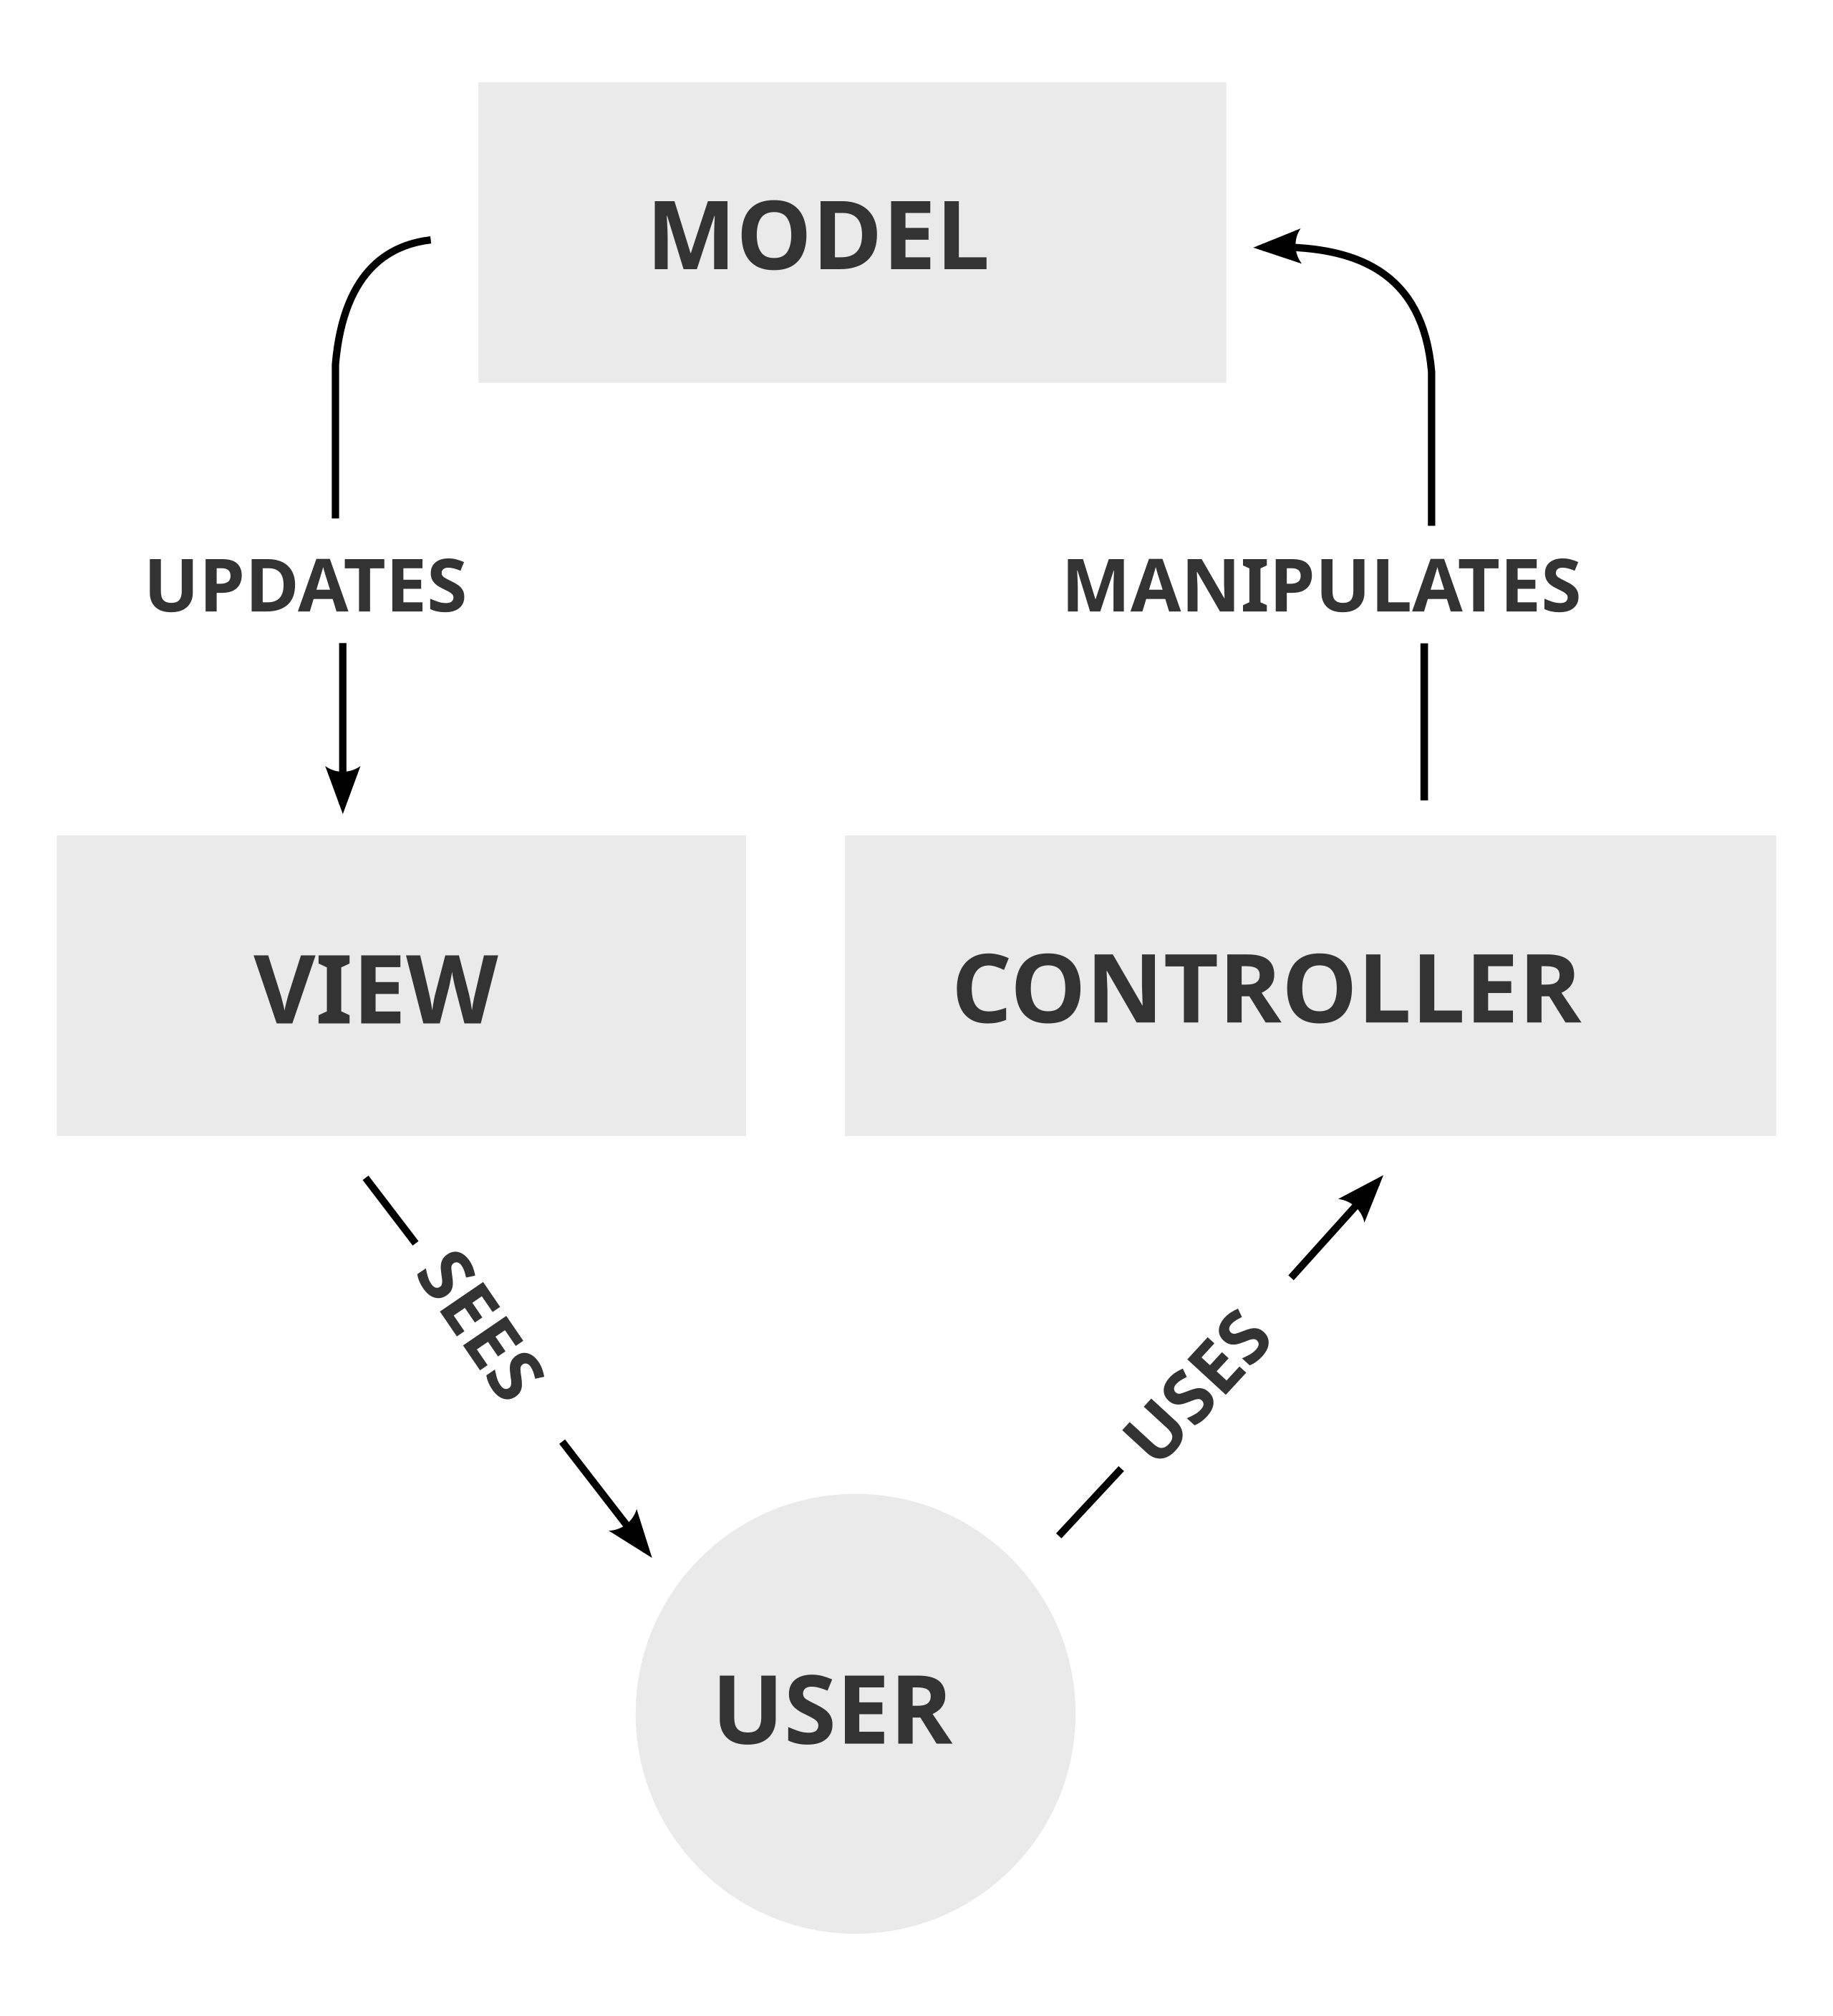
\includegraphics[width=0.8\textwidth]{mvc}
      \end{figure}
    \end{column}
  \end{columns}
\end{frame}

\section{Docker (extra)}
\begin{frame}
  \frametitle{Docker Introduction}
  \vspace*{-1.5ex}
  \pause
  \begin{block}{The problem}
    \begin{itemize}
      \item Software depends on specific versions of system libraries, and in the computer environment in general (e.g. directory structures, databases, ambient variables, etc)
            \pause
      \item I use Linux, you may use Windows, your next group colleague may use MacOS
            \pause
      \item How do we make sure everybody has the exact same environment?
    \end{itemize}
    \pause
  \vspace*{-2ex}
    \begin{columns}
      \begin{column}{.95\textwidth}
        \begin{block}{Solution}
          \begin{itemize}
            \item We enforce the same environment in declarative manner: \\ version of system libraries, databases, the environment variables...
            \item Docker does exactly that!
          \end{itemize}
        \end{block}
      \end{column}
    \end{columns}
  \end{block}
  \vspace*{-1.8ex}
  \pause
  \begin{columns}
    \begin{column}{.45\textwidth}
  \begin{block}{What is Docker?}
    \begin{itemize}
            \pause
      \item What Docker is not: A virtual machine
            \pause
      \item It is a container solution based on a Linux kernel feature called cgroups
      \item It is also runs on MacOS and Windows
    \end{itemize}
  \end{block}
    \end{column}
    \pause
    \begin{column}{.45\textwidth}
      \begin{block}{Why use Docker?}
        \begin{itemize}
          \item Like git, it is a standard in the industry
          \item It will make the life of the TAs way easier
        \end{itemize}
      \end{block}
    \end{column}
  \end{columns}
\end{frame}

\begin{frame}[fragile]
  \frametitle{Docker basics}
  \pause
  \begin{block}{More concepts}
    \begin{itemize}
      \item Docker container: isolated process with its own file system
      \item Docker image: is a package that includes all of the files, binaries, libraries, and configurations to run a Docker container
            \begin{itemize}
              \item Built on layers: make your own image on top of existing ones
            \end{itemize}
            \item Docker volume: persistent data stores for containers
    \end{itemize}
  \end{block}
  \pause
  \begin{block}{An usual setup:}
    \begin{itemize}
      \item \texttt{Dockerfile}: The Docker image in which you main app will run on
      \item \texttt{entrypoint.sh}: The script that the Dockerfile calls when its container is starting up
      \item \texttt{docker-compose.yml}: Organizes all the different Docker container of your application
    \end{itemize}
  \end{block}
\end{frame}

\section{A Minimal MVC Flask app with Docker Project}
\begin{frame}
  \frametitle{A Minimal MVC Flask app with Docker Project}
  \begin{itemize}
    \item App
  \end{itemize}
\end{frame}

\section{Let's write our web apps!}
\begin{frame}
  \frametitle{Hands-on}
  \begin{itemize}
    \item Follow my step-by-step guide: \url{https://github.com/rafaelcgs10/dis2025}
    \item Follow the official Flask tutorial: \url{https://flask.palletsprojects.com/en/stable/tutorial/}
  \end{itemize}
\end{frame}

\end{document}
